\documentclass[12pt,journal,onecolumn]{IEEEtran}
\usepackage{graphicx}
\usepackage{longtable}

\begin{document}

\title{Task 3: Architectural Tactics and Patterns}
\author{Team 27}
\maketitle

\section{Goal and Scope}

This document explains how our architecture satisfies NFR1 to NFR6 for the coding practice platform.

MongoDB is selected as primary data storage as per ADR 005 in Task 2.

It includes:
\begin{itemize}
    \item practical implementation plan
    \item architectural tactics mapped to NFRs
    \item two implementation patterns
    \item diagram references with image files
\end{itemize}

\section{Implementation Plan for All NFRs}

\subsection{NFR1 Performance}
\textbf{Target}
\begin{itemize}
    \item code evaluation result in 5 seconds for normal case
    \item page response in 2 seconds
\end{itemize}

\textbf{Implementation}
\begin{enumerate}
    \item Use async pipeline. API pushes job to queue and worker handles execution.
    \item Cache question metadata and dashboard summary for short time.
    \item Add MongoDB indexes on user\_id, test\_id, submission\_id and created\_at.
    \item Keep baseline warm workers to reduce startup delay.
    \item Keep clear timeout for API calls and code execution.
\end{enumerate}

\textbf{Why it works}
\begin{itemize}
    \item API thread does not wait for compile or run
    \item cache and MongoDB indexes reduce repeated query load
    \item warm workers reduce end to end delay
\end{itemize}

\textbf{Check metrics}
\begin{itemize}
    \item p95 API latency under 2 seconds
    \item p95 evaluation completion under 5 seconds
\end{itemize}

\subsection{NFR2 Scalability}
\textbf{Target}
\begin{itemize}
    \item handle 1000 concurrent submissions
\end{itemize}

\textbf{Implementation}
\begin{enumerate}
    \item Scale app instances and worker instances horizontally.
    \item Separate queue routing by job type like code, SQL and MCQ.
    \item Auto scale worker count based on queue depth and CPU.
    \item Use MongoDB connection pooling and move heavy analytics to background jobs.
    \item Add backpressure using per user rate limits during overload.
\end{enumerate}

\textbf{Why it works}
\begin{itemize}
    \item queue absorbs spike traffic
    \item workers can be added without code change
    \item backpressure prevents full system collapse
\end{itemize}

\textbf{Check metrics}
\begin{itemize}
    \item stable p95 latency under load test
    \item no major error spike at peak load
\end{itemize}

\subsection{NFR3 Security}
\textbf{Target}
\begin{itemize}
    \item token based authentication
    \item sandbox execution with 256 MB RAM and 1 CPU core limits
\end{itemize}

\textbf{Implementation}
\begin{enumerate}
    \item JWT based auth with role checks for admin routes.
    \item Password hash using bcrypt or Argon2.
    \item Run code in isolated container with CPU, RAM and timeout limits.
    \item Disable container network unless needed.
    \item Add request validation, login rate limit and audit logging.
\end{enumerate}

\textbf{Why it works}
\begin{itemize}
    \item unauthorized access is blocked by token and role check
    \item untrusted code stays inside sandbox boundary
    \item rate limit and input validation reduce abuse
\end{itemize}

\textbf{Check metrics}
\begin{itemize}
    \item all protected routes require valid token
    \item all code jobs run with enforced resource limits
\end{itemize}

\subsection{NFR4 Availability}
\textbf{Target}
\begin{itemize}
    \item 99.5 percent uptime
\end{itemize}

\textbf{Implementation}
\begin{enumerate}
    \item Keep multiple app and worker instances.
    \item Use health checks and auto restart for unhealthy instance.
    \item Use bounded retry with exponential backoff.
    \item Use circuit breaker for unstable dependencies.
    \item Keep backup, restore drill and incident runbook.
\end{enumerate}

\textbf{Why it works}
\begin{itemize}
    \item no single instance failure should stop system
    \item retries handle temporary errors
    \item circuit breaker prevents cascading timeout
\end{itemize}

\textbf{Check metrics}
\begin{itemize}
    \item monthly uptime at or above 99.5 percent
    \item restore drill success rate in planned tests
\end{itemize}

\subsection{NFR5 Usability}
\textbf{Target}
\begin{itemize}
    \item student should start test in 3 clicks
\end{itemize}

\textbf{Implementation}
\begin{enumerate}
    \item Keep start flow simple: select config, start test, answer question.
    \item Keep same layout style in student and admin panels.
    \item Show inline validation and clear loading state.
    \item Keep keyboard access and mobile friendly layout.
    \item Run small user testing with first time users.
\end{enumerate}

\textbf{Why it works}
\begin{itemize}
    \item low click count reduces friction
    \item clear feedback reduces user confusion
\end{itemize}

\textbf{Check metrics}
\begin{itemize}
    \item test start success above 90 percent for new users
    \item average clicks to start test at or below 3
\end{itemize}

\subsection{NFR6 Maintainability}
\textbf{Target}
\begin{itemize}
    \item one module change should have minimal impact on others
\end{itemize}

\textbf{Implementation}
\begin{enumerate}
    \item Keep modular monolith boundaries: auth, test, evaluation and analytics.
    \item Keep layered structure inside each module: controller, service and repository.
    \item Keep versioned API and message contracts.
    \item Add unit tests, integration tests and CI quality checks.
    \item Keep ADR docs and structured logs.
\end{enumerate}

\textbf{Why it works}
\begin{itemize}
    \item module boundaries reduce side effects
    \item contract first approach reduces integration break
    \item tests catch regressions early
\end{itemize}

\textbf{Check metrics}
\begin{itemize}
    \item lower change failure rate
    \item stable CI pass trend
\end{itemize}

\section{Architectural Tactics}

\subsection{Tactic 1: Asynchronous Queue Processing}
\begin{itemize}
    \item Description: API publishes submission jobs and workers process in background.
    \item NFR mapping: NFR1, NFR2, NFR4.
    \item Reason: Decouples heavy processing from request path.
\end{itemize}

\subsection{Tactic 2: Sandbox Isolation}
\begin{itemize}
    \item Description: Execute code in isolated container with strict limits.
    \item NFR mapping: NFR3, NFR4.
    \item Reason: Untrusted code cannot impact host system.
\end{itemize}

\subsection{Tactic 3: Caching and Query Optimization}
\begin{itemize}
    \item Description: Cache hot reads and tune MongoDB indexes and queries.
    \item NFR mapping: NFR1, NFR2.
    \item Reason: Reduces repeated expensive query work.
\end{itemize}

\subsection{Tactic 4: Retry, Circuit Breaker and Health Checks}
\begin{itemize}
    \item Description: Use bounded retry, failure isolation and automated health monitoring.
    \item NFR mapping: NFR4, NFR2.
    \item Reason: Prevents cascading failures during dependency issues.
\end{itemize}

\subsection{Tactic 5: Modular Monolith with Stable Contracts}
\begin{itemize}
    \item Description: Keep clear module boundaries and stable interfaces.
    \item NFR mapping: NFR6, NFR2, NFR5.
    \item Reason: Easier updates, better team parallel work and safer integration.
\end{itemize}

\section{Implementation Patterns}

\subsection{Pattern 1: Strategy Pattern}
\textbf{Role in architecture}
\begin{itemize}
    \item EvaluationController selects strategy based on submission type.
    \item MCQStrategy, SQLStrategy and CodeStrategy keep logic separate.
    \item New evaluator can be added without changing core controller flow.
\end{itemize}

\textbf{Why this pattern}
\begin{itemize}
    \item avoids large conditional blocks
    \item easy extension for new question types
    \item unit testing is easy because each strategy is isolated
\end{itemize}

\begin{figure}[htbp]
\centering
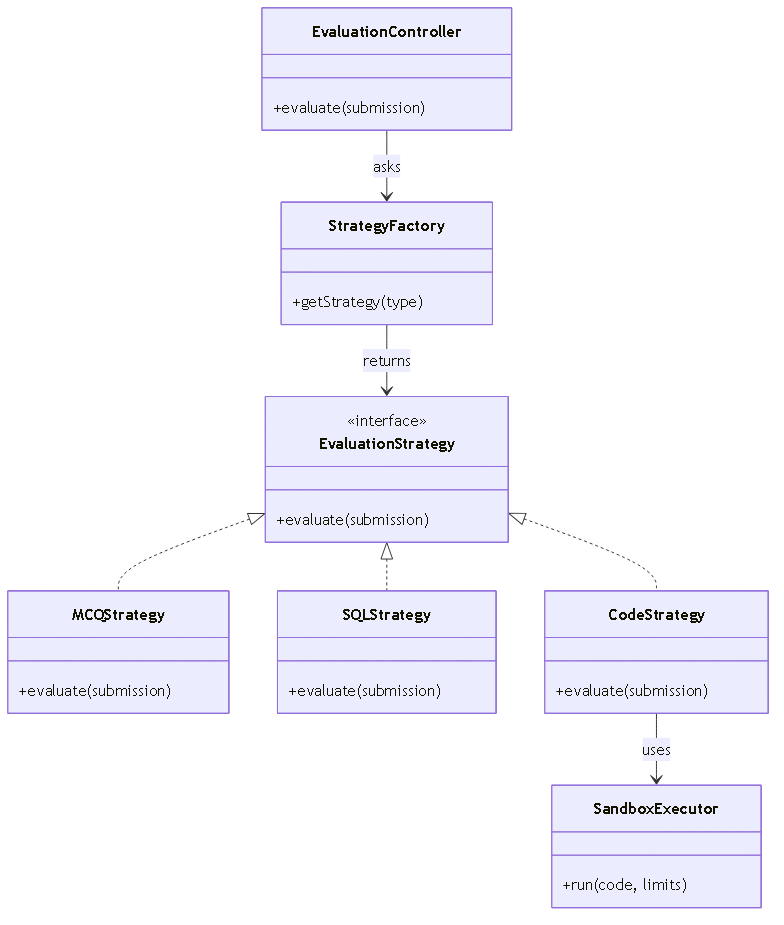
\includegraphics[width=0.95\linewidth]{diagrams/task3-uml-strategy.png}
\caption{Task 3 UML strategy pattern}
\label{fig:task3-strategy}
\end{figure}

Diagram source: \texttt{diagrams/task3-uml-strategy.mmd}

\subsection{Pattern 2: Factory Method Pattern}
\textbf{Role in architecture}
\begin{itemize}
    \item StrategyFactory creates evaluator objects.
    \item Controller asks factory and does not create concrete classes directly.
    \item If new evaluator type is added only factory mapping changes.
\end{itemize}

\textbf{Why this pattern}
\begin{itemize}
    \item central creation logic
    \item lower coupling between controller and concrete classes
\end{itemize}

\begin{figure}[htbp]
\centering
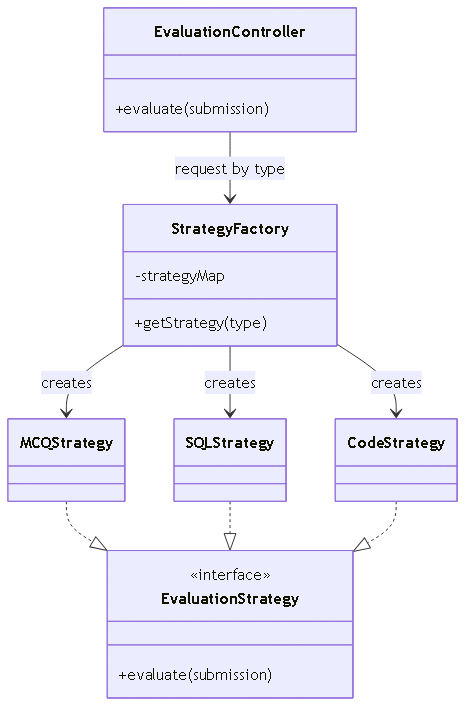
\includegraphics[width=0.95\linewidth]{diagrams/task3-uml-factory.png}
\caption{Task 3 UML factory pattern}
\label{fig:task3-factory}
\end{figure}

Diagram source: \texttt{diagrams/task3-uml-factory.mmd}

\section{Architectural Patterns Used in System}

\subsection{Client Server Pattern}
\begin{itemize}
    \item Use: Browser clients call backend APIs.
    \item Why fit: UI and business logic stay separate.
    \item NFR impact: NFR5, NFR6.
\end{itemize}

\subsection{Layered Architecture Pattern}
\begin{itemize}
    \item Use: API layer, service layer and data layer in each module.
    \item Why fit: Easier change and easier testing.
    \item NFR impact: NFR6, NFR3.
\end{itemize}

\subsection{MVC Pattern in Frontend}
\begin{itemize}
    \item Use: View for UI, controller for actions, model for state.
    \item Why fit: UI changes do not break data logic.
    \item NFR impact: NFR5, NFR6.
\end{itemize}

\subsection{Event Driven Pattern}
\begin{itemize}
    \item Use: Submission events go to queue and workers consume jobs.
    \item Why fit: Better burst handling and low coupling.
    \item NFR impact: NFR1, NFR2, NFR4.
\end{itemize}

\subsection{Modular Monolith Pattern}
\begin{itemize}
    \item Use: Single deployable app with strict module boundaries.
    \item Why fit: Less ops complexity for current team size and timeline.
    \item NFR impact: NFR6, NFR2, NFR4.
\end{itemize}

\section{System Diagrams}

\subsection{C4 Style Container View}
\begin{figure}[htbp]
\centering
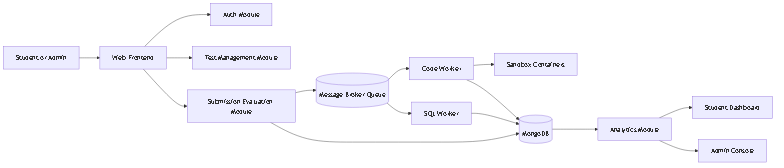
\includegraphics[width=0.95\linewidth]{diagrams/task3-c4-container.png}
\caption{Task 3 C4 container view}
\label{fig:task3-c4}
\end{figure}

Diagram source: \texttt{diagrams/task3-c4-container.mmd}

\subsection{UML Strategy and Factory Overview}
\begin{figure}[htbp]
\centering
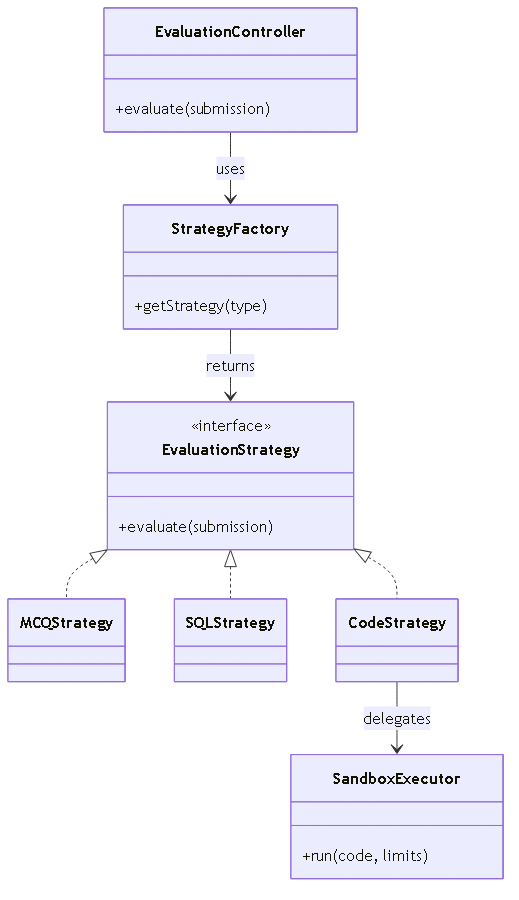
\includegraphics[width=0.95\linewidth]{diagrams/task3-uml-strategy-factory-overview.png}
\caption{Task 3 UML strategy and factory overview}
\label{fig:task3-overview}
\end{figure}

Diagram source: \texttt{diagrams/task3-uml-strategy-factory-overview.mmd}

\section{NFR to Tactic Traceability Matrix}

\begin{longtable}{|p{3cm}|p{6cm}|p{5cm}|}
\hline
\textbf{NFR} & \textbf{Main Tactics} & \textbf{Supporting Patterns} \\
\hline
NFR1 Performance & Async queue, caching, MongoDB tuning & Event Driven and Strategy \\
\hline
NFR2 Scalability & Horizontal scaling, queue routing, backpressure & Event Driven and Modular Monolith \\
\hline
NFR3 Security & Sandbox, token auth, rate limiting & Layered Architecture and Strategy \\
\hline
NFR4 Availability & Redundancy, retry, circuit breaker, health checks & Event Driven and Modular Monolith \\
\hline
NFR5 Usability & Simple flow, consistent UI, clear feedback & MVC and Client Server \\
\hline
NFR6 Maintainability & Modular boundaries, stable contracts, CI checks & Layered Architecture with Strategy and Factory Method \\
\hline
\end{longtable}

\section{Recommended Implementation Order}

\begin{enumerate}
    \item Build auth and sandbox baseline first.
    \item Add queue pipeline and worker pool.
    \item Add reliability controls like retry and circuit breaker.
    \item Add cache and MongoDB optimization.
    \item Improve UX flow and run user testing.
    \item Strengthen CI, tests and documentation.
\end{enumerate}

This sequence reduces security risk first then improves speed, scale and long term maintainability.

\end{document}
